% ========== Documentation-Template modified by Gökmen Kiyan (goekmen.kiyan@stud.fh-campuswien.ac.at) in 2023 =============

% ========== Issues may occur! Use this template at your own risk. =============

\documentclass[a4paper,12pt,numbers=noenddot]{scrreprt}
\usepackage[left= 3.5cm,right = 3cm, bottom = 3cm, top = 3cm]{geometry}
\usepackage[onehalfspacing]{setspace}

% ============= Settings for the document =============
\def\workTitle{Dokumententitel}
\def\subTitle{Untertitel}
\def\specialization{Titel der Vorlesung}
\def\studentFirstNameone{Vorname}
\def\studentLastNameone{Nachname}
\def\studentIdone{xx000000}
\def\studentFirstNametwo{Vorname}
\def\studentLastNametwo{Nachname}
\def\studentIdtwo{xx000001}
\def\advisorPreTitle{Vorg.-Titel}
\def\advisoFirstName{Vorname}
\def\advisorLastName{Nachname}
\def\advisorPosTitle{Nachg. Titel}
\def\assessorPreTitle{Vorg.-Titel}
\def\assessorFirstName{Vorname}
\def\assessorLastName{Nachname}
\def\assessorPosTitle{Nachg. Titel}
\def\dateDay{\the\day}
\def\dateMonth{\the\month}
\def\dateYear{\the\year}

%===================================================
% Switch between commands 
% German or English version
\newif\ifuseGermanVersion	
% Departments
\newif\ifuseAllgemein
\newif\ifuseComputerScience
%===================================================


% Switch between englich and german be using the %.
%\useGermanVersiontrue % German version
\useGermanVersionfalse % English version

% Choose your department be using the %.
% \useAllgemeintrue % Default template
\useComputerSciencetrue % Computer Science

% ============= Packages =============

% Switch between German and English such as the title page design based on the main.tex. file settings
\usepackage{ifthen}

% Switch the Language (automatic)
\ifuseGermanVersion
	\usepackage[ngerman]{babel}	% German
\else
	\usepackage[english]{babel} % English
\fi

% Standard Packages
\usepackage[utf8]{inputenc}
\usepackage{graphicx} % Used to insert images
\usepackage{float} %Package for using the [H] option on graphics to force them into place
\usepackage[export]{adjustbox} % Used to constrain images to a maximum size
\usepackage{enumerate} % Needed for markdown enumerations to work
\usepackage{geometry} % Used to adjust the document margins
\usepackage{amsmath} % Equations
\usepackage{amssymb} % Equations
\usepackage[mathletters]{ucs} % Extended unicode (utf-8) support
\usepackage{fancyvrb} % verbatim replacement that allows latex
\usepackage{grffile} % extends the file name processing of package graphics
\usepackage{url}
\def\UrlBreaks{\do\/\do-}
\usepackage{hyperref}
\usepackage{longtable} % longtable support required by pandoc >1.10
\usepackage{multicol}
\usepackage{multirow}
\usepackage[nohyperlinks]{acronym}
\usepackage{enumitem}
\usepackage{fixmath}
%\usepackage{showframe}
\usepackage{blindtext}
\usepackage[T1]{fontenc}
\usepackage{graphicx}
\usepackage{subfigure}
\graphicspath{{Figures/}} % define path of images
\usepackage{animate}
\usepackage{fancyhdr}
\usepackage{lmodern}
\usepackage[dvipsnames]{xcolor}
\usepackage{footnote}
\usepackage{lastpage}

% Citation style
\usepackage{natbib}
\bibliographystyle{apalike}

% BlockDiagram Drawing Package
\usepackage{tikz}
\usetikzlibrary{shapes,arrows}
\usepackage[european,nooldvoltagedirection]{circuitikz}
\usepackage{pgfplots}
\pgfplotsset{compat=1.10}
\usepackage{mathtools}
\usepackage{pgf-pie}
\usepackage{textcomp}
\usepackage{pgfplots}
\usepgfplotslibrary{statistics}
\usepackage{smartdiagram}

%  ============= Ubuntu Code Block Style Config =============

% Ubuntu Style Code
\definecolor{mygreen}{rgb}{0,0.6,0}
\definecolor{mygray}{rgb}{0.5,0.5,0.5}
\definecolor{mymauve}{rgb}{0.58,0,0.82}
\definecolor{terminalbgcolor}{HTML}{330033}
\definecolor{terminalrulecolor}{HTML}{000099}
\newcommand{\lstconsolestyle}{
\lstset{
	backgroundcolor=\color{terminalbgcolor},
	basicstyle=\color{white}\fontfamily{fvm}\footnotesize\selectfont,
	breakatwhitespace=false,  
	breaklines=true,
	captionpos=b,
	commentstyle=\color{mygreen},
	deletekeywords={...},
	escapeinside={\%*}{*)},
	extendedchars=true,
	frame=single,
	keepspaces=true,
	keywordstyle=\color{blue},
	%language=none,
	morekeywords={*,...},
	numbers=none,
	numbersep=5pt,
        framerule=2pt,
	numberstyle=\color{mygray}\tiny\selectfont,
	rulecolor=\color{terminalrulecolor},
	showspaces=false,
	showstringspaces=false,
	showtabs=false,
	stepnumber=2,
	stringstyle=\color{mymauve},
	tabsize=2
}
}

%  =============  =============

%  ============= BlockDiagram Drawing Config =============
% Definition of blocks:
\tikzset{%
  block/.style    = {draw, thick, rectangle, minimum height = 3em,
    minimum width = 3em},
  sum/.style      = {draw, circle, node distance = 2cm}, % Adder
  input/.style    = {coordinate}, % Input
  output/.style   = {coordinate}, % Output
  mult/.style	  = {draw, isosceles triangle, minimum height=1cm, minimum width =1cm}
}

%  ============= Settings for listings  =============
\usepackage{listings,lstautogobble}
\lstset{title=\lstname, frame=single, framerule=0pt, rulecolor=\color{lightgray}, showspaces=false, showstringspaces=false, showtabs=false, numbers=left, numbersep=5pt, numberstyle=\sffamily\tiny\color{gray}, breaklines=false, autogobble=true, basicstyle=\sffamily\scriptsize}

\usepackage[breakable]{tcolorbox}
\newtcolorbox{codeblock}{
    colback=gray!5!white,
    colframe=gray!95!black,
    before skip=20pt,
    after skip=20pt
    }
\newtcolorbox{codeblock-b}{
    breakable,
    colback=gray!5!white,
    colframe=gray!95!black,
    before skip=20pt,
    after skip=20pt
    }
\newtcolorbox{box-black}{
    colback=black,
    colframe=black,
    before skip=10pt,
    after skip=10pt
    }

%  ============= Color definition ============= 
% FH-Blau
\definecolor{FH}{RGB}{0, 84, 150}

\ifuseAllgemein
    % FH-Farbe 2
    \definecolor{FH2}{RGB}{0, 84, 150}
\fi

\ifuseComputerScience
    % FH-Farbe 2
    \definecolor{FH2}{RGB}{38, 102, 181}
\fi

% ============= No massive space betweend headline and chapter titel =============
\renewcommand*{\chapterheadstartvskip}{\vspace*{-.4cm}}
\renewcommand*{\chapterheadendvskip}{\vspace{.5cm}}

\setlength{\parindent}{0pt} % no indent at paragraph start

% ============= Header and Footer =============
\renewcommand{\chaptermark}[1]{\markboth{\thechapter~ #1}{}}

\fancypagestyle{icmt-fancy}{%
  \fancyhf{}% Clear header and footer
  %\fancyhead[L]{\leftmark}
  \fancyhead[L]{\subTitle}
  \fancyhead[R]{}
  \fancyfoot[L]{\studentLastNameone~|~\studentLastNametwo}
  \fancyfoot[R]{\thepage}% Custom footer *~|~\pageref{LastPage}
  \renewcommand{\headrulewidth}{0.4pt}% Line at the header visible
  \renewcommand{\footrulewidth}{0.4pt}% Line at the footer visible
}

% Define horizontal lines above and below the main content
\makeatletter
\def\thickhline{%
	\noalign{\ifnum0=`}\fi\hrule \@height \thickarrayrulewidth \futurelet
	\reserved@a\@xthickhline}
\def\@xthickhline{\ifx\reserved@a\thickhline
	\vskip\doublerulesep
	\vskip-\thickarrayrulewidth
	\fi
	\ifnum0=`{\fi}}
\makeatother
\newlength{\thickarrayrulewidth}
\setlength{\thickarrayrulewidth}{2\arrayrulewidth}

% ============= Redefine the plain page style =============
\fancypagestyle{plain}{%
  \fancyhf{}%
  \fancyfoot[R]{\thepage}%
  \renewcommand{\headrulewidth}{0.0pt}% Line at the header invisible
  \renewcommand{\footrulewidth}{0.0pt}% Line at the footer visible
}
\renewcommand*{\chapterpagestyle}{icmt-fancy}

% ============= Size of headings =============
\setkomafont{chapter}{\LARGE}
\setkomafont{section}{\Large}
\setkomafont{subsection}{\large}
\setkomafont{subsubsection}{\normalsize}
\setkomafont{paragraph}{\normalsize}
\setkomafont{subparagraph}{\small}

% roman numbering with \RM{Zahl}
\newcommand{\RM}[1]{\MakeUppercase{\romannumeral #1}}

% ============= hyperref should always be added at the end =============
\usepackage{hyperref}

\hypersetup{
    unicode=false, % non-Latin characters in Acrobat’s bookmarks
    pdftoolbar=true, % show Acrobat’s toolbar?
    pdfmenubar=true, % show Acrobat’s menu?
    pdffitwindow=false, % window fit to page when opened
    pdfstartview={FitV}, % fits the width of the page to the window
    pdfpagelayout={SinglePage}, % displays only one page when opened in pdf viewer
    pdftitle={\workTitle},
	pdfsubject={\subTitle},
	pdfauthor={\studentFirstNameone~\studentLastNameone,~\studentFirstNametwo~\studentLastNametwo},
	pdfkeywords={\workTitle,~\subTitle,~\specialization},
    pdfcreator={pdflatex}, % creator of the document
    pdfproducer={LaTeX with hyperref}, % producer of the document
    pdfnewwindow=true, % links in new window
    colorlinks=false, % false: boxed links; true: colored links
    linkcolor=black, % color of internal links (change box color with linkbordercolor)
    citecolor=black, % color of links to bibliography
    filecolor=black, % color of file links
 	breaklinks=true,	
	menucolor=black,
    urlcolor=black % color of external links
}

% ============= Begin of the main document =============
\begin{document}
% Title Page will change automatic
\ifuseGermanVersion 
	\newgeometry{left=2.4cm,right=2.4cm,bottom=2.5cm,top=2cm}

% first titlepage
\pagestyle{empty}

\begin{figure}[H]
\vspace*{-2.5cm}
\ifuseMedienundDigitaleTechnologien
\hspace*{2.7cm}
	
\includegraphics[keepaspectratio, width=1.4\textwidth, right]{TemplateElements/fh_campus_header.png}
\fi
\end{figure}


\begin{center}
\vspace{2cm}
\begin{minipage}[t][5cm][s]{\textwidth}%
\centering
\Huge{{\color{FH2}{\fontsize{24}{30} \textbf{\sffamily{\workTitle}}\\}}}
\vspace{0.5cm}
\LARGE{{\color{FH2}{\fontsize{16}{24} \textbf{\sffamily{\subTitle}}\\}}}
\vspace{0.5cm}
\LARGE{{\color{FH2}{\fontsize{14}{22} \textbf{\sffamily{\specialization}}}}}
\end{minipage}

\vfill

Ausgeführt von:\\ 
\fontsize{15pt}{15pt}\selectfont
\textbf{\sffamily{\studentFirstNameone\ \studentLastNameone}} \\
\fontsize{11pt}{15pt}\selectfont
\studentIdone\\

\fontsize{15pt}{15pt}\selectfont
\textbf{\sffamily{\studentFirstNametwo\ \studentLastNametwo}} \\
\fontsize{11pt}{15pt}\selectfont
\studentIdtwo\\

\vfill

\begin{tabular}{lll}
Vortragender: & \advisorPreTitle\ \advisoFirstName\ \advisorLastName, \advisorPosTitle \\
Begutachter: & \assessorPreTitle\ \assessorFirstName\ \assessorLastName, \assessorPosTitle
\end{tabular}

\vfill

\normalsize{\dateDay.\dateMonth.\dateYear}

\end{center}
\restoregeometry
\else
	\newgeometry{left=2.4cm,right=2.4cm,bottom=2.5cm,top=2cm}

% first titlepage
\pagestyle{empty}

\begin{figure}[H]
\vspace*{-2.5cm}
\ifuseComputerScience
\hspace*{2.7cm}
	
\includegraphics[keepaspectratio, width=1.4\textwidth, right]{TemplateElements/fh_campus_header.png}
\end{figure}

\begin{center}
\vspace{2cm}
\begin{minipage}[t][5cm][s]{\textwidth}%
\centering
\Huge{{\color{FH2}{\fontsize{24}{30} \textbf{\sffamily{\workTitle}}\\}}}
\vspace{0.5cm}
\LARGE{{\color{FH2}{\fontsize{16}{24} \textbf{\sffamily{\subTitle}}\\}}}
\vspace{0.5cm}
\LARGE{{\color{FH2}{\fontsize{14}{22} \textbf{\sffamily{\specialization}}}}}
\end{minipage}

\vfill

Submitted by:\\
\fontsize{15pt}{15pt}\selectfont
\textbf{\sffamily{\studentFirstNameone\ \studentLastNameone}} \\
\fontsize{11pt}{15pt}\selectfont
\studentIdone\\
\fontsize{15pt}{15pt}\selectfont
\textbf{\sffamily{\studentFirstNametwo\ \studentLastNametwo}} \\
\fontsize{11pt}{15pt}\selectfont
\studentIdtwo\\

\vfill

\begin{tabular}{lll}
Lecturer: & \advisorPreTitle\ \advisoFirstName\ \advisorLastName, \advisorPosTitle \\
Assessor: & \assessorPreTitle\ \assessorFirstName\ \assessorLastName, \assessorPosTitle
\end{tabular}

\vfill

\normalsize{\dateDay.\dateMonth.\dateYear}


\end{center}

\restoregeometry
\fi

\chapter*{Abkürzungsverzeichnis}
\begin{acronym}
	\acro{fh}[FH]{Fachhochschule}
\end{acronym}
\pagenumbering{Roman} % roman page numbering

% Table of content
\setcounter{tocdepth}{1} % Levels in the table of content
\tableofcontents
\cleardoubleemptypage
\pagenumbering{arabic} % arabic page numbering

\setlist[enumerate,1]{label*=\arabic*.,font=\bfseries\sffamily}

\pagestyle{icmt-fancy}
% ================================
% =            CONTENT           =
% ================================
\chapter{Einführung \LaTeX}
\LaTeX~ermöglicht das Erstellen eines einheitlichen Dokuments mit nur wenigen Grundeinstellungen. Es erlaubt jedoch auch eine benutzerdefinierte Formatierung bis hin zum kleinsten Detail eines Dokumentes. Anhand des kurzen Einführungskapitels soll auf die wichtigsten Grundfunktionen eingegangen werden.

\section{Grundformatierung}
Im Textbearbeitungsprogramm \LaTeX~wird zwischen folgenden Untergliederungsstufen unterschieden:
\begin{itemize}
	\item \verb|\chapter{Kapitel}|
	\item \verb|\section{Unterkapitel}|
	\item \verb|\subsection{Unterunterkapitel}|
	\item \verb|\subsubsection{Unterunterunterkapitel}|
	\item \verb|\paragraph{Paragraph}|
	\item \verb|\subparagraph{Unterparagraph}|
\end{itemize}

Eine Untergliederung ist jedoch nur bis zur \verb|\subsection{Titel}| sinnvoll. In Einzelfällen kann eine weitere Gliederungsstufe \verb|\subsubsection{Titel}| notwendig werden. Diese wird dann aber nichtmehr im Inhaltsverzeichnis aufgelistet.\\

Abstände werden grundsätzlich von \LaTeX~selbst gesetzt und müssen nicht extra hinzugefügt werden. Sollte es dennoch so sein das man Abstände erzwingen möchte so funktioniert das entweder mit \verb|\newline| oder \verb|\\|.

\section{Aufzählungen}
Aufzählungen können ganz einfach mit
\begin{verbatim}
\begin{itemize}
   \item Aufzählungspunkt 1
   \item Aufzählungspunkt 2
\end{itemize}
\end{verbatim}
eingefügt werden.\pagebreak

Das Ergebnis sieht dann wie folgt aus:
\begin{itemize}
	\item Aufzählungspunkt 1
	\item Aufzählungspunkt 2
\end{itemize}
Wird \verb|itemize| mit \verb|enumerate| ausgetauscht so werden statt Aufzählungspunkten entsprechende Zahlen ausgegeben. Die Nummerierung beginn in der Regel bei \verb|1.|.

\section{Abbildungen}
Abbildungen können entweder mit dem im Editor vorhandenen Assistenten eingefügt oder manuell über folgende Zeilen:

\begin{verbatim}
\begin{figure}[H]
	\centering
	\includegraphics[width=0.6\linewidth]{fh_campus}
	\caption{\acs{fh} wird zum Campus St. Pölten~\cite{fhcampus_link}}
	\label{fig:fhcampus}
\end{figure}
\end{verbatim}

Das Ergebnis sieht dann wie folgt aus:
\begin{figure}[H]
	\centering
	\includegraphics[width=0.6\linewidth]{Figures/fh_campus}
	\caption{\acs{fh} Campus Wien~\cite{fhcampus_link}}
	\label{fig:fhcampus}
\end{figure}
Mit \verb|[width=0.6\linewidth]| wird beispielsweise die Breite des Bildes auf 60\% der Gesamttextbreite festgelegt. \verb|\caption{Bildunterschrift}| definiert eine Bildunterschrift, \verb|\label{fig:fhcampus}| ermöglicht das Referenzieren des Bildes im Text.

Beispielsweise könnte die Referenzierung wie folgt aussehen:

\textit{In der Abbildung \ref{fig:fhcampus} ist das neue Campusgebäude der FH Campus Wien zu sehen.}
\pagebreak

\section{Tabellen}
Tabellen erweitern die Komplexitätsstufe der manuellen Erstellung erheblich. Für das grobe Layout empfiehlt sich grundsätzlich der Tabellenassistent. Für eine feinere beziehungsweise spezielle Formatierung muss händisch nachgearbeitet werden.

\begin{table}[H]
	\begin{tabular}{|c|c|c|c|c|c|}
		\hline 
		\multirow{2}{*}{\sffamily{\textbf{Wert}}} & \sffamily{\textbf{Metallschicht}} & \multicolumn{2}{c|}{\multirow{2}{*}{\sffamily{\textbf{Toleranzbereich}}}} & \multirow{2}{*}{\sffamily{\textbf{Messwert}}} & \multirow{2}{*}{\sffamily{\textbf{Im Toleranzbereich}}} \\
		& \sffamily{\textbf{Toleranzfarbe}} & \multicolumn{2}{c|}{} & & \\
		\thickhline
		$510~\Omega$ & Braun & $515.1~\Omega$ & $504.9~\Omega$ & $506~\Omega$ & \textcolor{green}{$\checkmark$} \\ 
		\hline
		$4.7~k\Omega$ & Braun & $4747~\Omega$ & $4653~\Omega$ & $4650~\Omega$ & {\Large \textcolor{red}{$\times$}} \\ 
		\hline 
		$100~k\Omega$ & Braun & $101~k\Omega$ & $99~k\Omega$ & $100~k\Omega$ & \textcolor{green}{$\checkmark$} \\ 
		\hline 
	\end{tabular}
	\caption{Wertetabelle verschiedener Metallschichtwiderstände}
	\label{tab:metallschichwiderstaende}
\end{table}

Auch hier kann die Tabelle wieder im Text referenziert werden.

\textit{Aus der Tabelle \ref{tab:metallschichwiderstaende} geht klar heraus das sich der $4.7k\Omega$ Widerstand nicht im Toleranzbereich befindet.}

\section{Mathematische Formeln}
Recht beliebt ist auch die Möglichkeit mathematische Funktionen, Rechenschritte und Co direkt in \LaTeX~zu dokumentieren. Dazu unterscheidet man zwischen folgenden Definitionen:
\begin{description}
	\item[Inline] Hier wird die Formel direkt in der Zeile eingefügt. $ c = \sqrt{a^2 + b^2} $
	\item[displaymath] Die Formel wird hierbei in einer neuen Zeile mittig eingefügt. \begin{displaymath}
	c = \sqrt{a^2 + b^2}
	\end{displaymath}
	\item [equation] Auch hier wird die Formel mittig in einer separaten Zeile eingefügt, weiters erscheint am Rand eine fortlaufende Nummer. Diese kann wie bei Bildern oder Tabellen bekannt im Text referenziert werden.
	\begin{equation} \label{eq:quadratwurzel}
	c = \sqrt{a^2 + b^2}
	\end{equation}
\end{description}

\textit{Die Länge der Hypotenuse entspricht der Quadratwurzel aus der Summe der Kathetenquadrate, mathematisch ausgedrückt folgt daraus die Formel \ref{eq:quadratwurzel}.}

\section{Interessante Packages}
Mithilfe diverser Pakete lassen sich recht schön verschiedenste Objekte in \LaTeX~einbinden. Für diverse Anwendungsfälle existieren eigene Pakete, eine Internetrecherche führt mit den richtigen Suchbegriffen am schnellsten zur idealen Lösung.
\subsection*{tikz}
Mit \verb|tikz| lassen sich eine Vielzahl an Diagrammen im 2D als auch 3D Raum erstellen. 
\begin{figure}[H]
	\centering
	\begin{tikzpicture}
	\pie[sum=auto, radius=3, text=pin, color={yellow, cyan, red, magenta},after number=\%]
	{
		46.6/Chrome,
		24.6/Internet Explorer,
		20.4/Firefox,
		8.4/Other
	}
	\end{tikzpicture}
	\caption{Verwendete Browser laut Musterstudie XY}
\end{figure}

\begin{figure}[H]
	\centering
	\begin{tikzpicture}
	\begin{axis}[width=10cm,height=5cm,ylabel shift = .2cm,
	xlabel={Spannung in $V$},
	ylabel={Stromstärke in $mA$},
	xmin=0, xmax=12,
	ymin=0, ymax=24,
	xtick={0,2,4,6,8,10},
	ytick={0,4,8,12,16,20},
	log ticks with fixed point,
	%legend style={at={(0.5,-0.1)},anchor=north},
	legend columns=-2,
	legend entries={gemessen, berechnet},
	legend to name=named,
	ymajorgrids=true,
	xmajorgrids=true,
	grid style=dashed,
	/pgf/number format/.cd,
	use comma,
	1000 sep={},
	]
	
	\addplot [color=red, thick, mark=o]  coordinates {
		(2,3.87)
		(4,7.73)
		(6,11.59)
		(8,15.44)
		(10,19.29)
	};
	
	\addplot [color=blue, thick, mark=square] coordinates {
		(2,3.92)
		(4,7.84)
		(6,11.76)
		(8,15.69)
		(10,19.61)
	};
	\end{axis}
	\end{tikzpicture}
	\ref{named}
	\caption{Linearität der Stromstärke -- $510~\Omega$}
\end{figure}

\subsection*{listings}
Für die Dokumetation des Quellcodes steht das Paket \verb|listings| zur Verfügung.

Mit \verb|\lstinputlisting{Datei}| kann eine ganze Datei einfach in die Dokumentation eingebunden werden.

\lstset{language=Python,caption={Primzahlenevaluierung, \lstname},label=DescriptiveLabel}
\begin{codeblock}
	\lstinputlisting{Code/Exercise_Task_1.py}
\end{codeblock}

\subsection*{Ubuntu Style Block}
Für die Dokumentation eines Codeblocks im Style eines Ubuntu Terminals steht das Paket \verb|lstlisting| zur Verfügung. \\


\lstconsolestyle % Dieser Command muss in das jeweilige Textdokuemnte eingefügt werden
Mit \verb|\begin{lstlisting} ... \end{lstlisting}| kann ein Code-Snippet in die Dokumentation eingebunden werden.


\section{Verzeichnisse}
Eine anständige und ordentliche Dokumentation benötigt selbstverständlich entsprechende Verzeichnisse. Sei es ein Abbildungsverzeichnis \verb|\listoffigures|, ein Tabellenverzeichnis \verb|\listoftables|, Codeverzeichnisse \verb|\lstlistoflistings| oder ein Literaturverzeichnis. \LaTeX~erstellt diverse Verzeichnisse unabhängig davon ob sie benötigt werden oder nicht, eingebunden werden sie mit den im Text angeführten Befehlen. Das Literaturverzeichnis benötigt ein wenig Eigeninitiative. Abhängig von den entsprechenden Quellen sind andere Definitionen zu wählen.
\chapter{Kapitel 2}
\blindtext

\section{Unterkapitel 1}
\blindtext

\section{Unterkapitel 2}
\blindtext

\section{Unterkapitel 3}
\blindtext
 \chapter{Kapitel 3}
\blindtext
\section{Unterkapitel 1}
\blindtext
\section{Unterkapitel 2}
\blindtext
\section{Unterkapitel 3}
\blindtext
\begin{abstract}
	\LaTeX~ermöglicht das Erstellen professioneller Dokumentationen im großen Umfang. Eine Vielzahl von sogenannten \verb|packages| ermöglicht eine schier grenzenlose Gestaltung eines hoch professionellen Dokuments.\\
	
	Darüber hinaus können in \LaTeX~nicht nur Dokumentationen erstellt werden. Ein weiteres Anwendungsgebiet wären Präsentationen.\\
	
	Aufgrund der vielen Gestaltungsmöglichkeiten ist es schwer die Eine und Richtige Vorlage zu erstellen. Eine Vielzahl an Vorlagen sind auf diversen Webseiten zu finden. Auch kommt es speziell auf das Gebiet der Dokumentation an.\\
	
	Gerade für mathematische oder technische Dokumentationen wird \LaTeX~gerne verwendet. Aber selbst eine Softwaredokumentation lässt sich mit \LaTeX~ideal umsetzten. Mit diversen Werkzeugen kann direkt Sourcecode in die Dokumentation übernommen werden. Eine spezielle Formatierung ist dafür nicht notwendig. Möglich machen das die unzähligen \verb|packages|.
\end{abstract}

\pagestyle{icmt-fancy} 
% List of bibliography (displays cite elements)
\addcontentsline{toc}{chapter}{\bibname}
\bibliography{Bibliography}
\cleardoubleemptypage
%% List of figures
\addcontentsline{toc}{chapter}{\listfigurename}
\listoffigures
\cleardoubleemptypage
% List of tables
\addcontentsline{toc}{chapter}{\listtablename}
\listoftables
\cleardoubleemptypage
% List of code elements
\addcontentsline{toc}{chapter}{\lstlistingname}
\lstlistoflistings

\end{document}
% ============= End of the main document =============























